\documentclass{article}\usepackage[]{graphicx}\usepackage[]{color}
%% maxwidth is the original width if it is less than linewidth
%% otherwise use linewidth (to make sure the graphics do not exceed the margin)
\makeatletter
\def\maxwidth{ %
  \ifdim\Gin@nat@width>\linewidth
    \linewidth
  \else
    \Gin@nat@width
  \fi
}
\makeatother

\definecolor{fgcolor}{rgb}{0.345, 0.345, 0.345}
\newcommand{\hlnum}[1]{\textcolor[rgb]{0.686,0.059,0.569}{#1}}%
\newcommand{\hlstr}[1]{\textcolor[rgb]{0.192,0.494,0.8}{#1}}%
\newcommand{\hlcom}[1]{\textcolor[rgb]{0.678,0.584,0.686}{\textit{#1}}}%
\newcommand{\hlopt}[1]{\textcolor[rgb]{0,0,0}{#1}}%
\newcommand{\hlstd}[1]{\textcolor[rgb]{0.345,0.345,0.345}{#1}}%
\newcommand{\hlkwa}[1]{\textcolor[rgb]{0.161,0.373,0.58}{\textbf{#1}}}%
\newcommand{\hlkwb}[1]{\textcolor[rgb]{0.69,0.353,0.396}{#1}}%
\newcommand{\hlkwc}[1]{\textcolor[rgb]{0.333,0.667,0.333}{#1}}%
\newcommand{\hlkwd}[1]{\textcolor[rgb]{0.737,0.353,0.396}{\textbf{#1}}}%

\usepackage{framed}
\makeatletter
\newenvironment{kframe}{%
 \def\at@end@of@kframe{}%
 \ifinner\ifhmode%
  \def\at@end@of@kframe{\end{minipage}}%
  \begin{minipage}{\columnwidth}%
 \fi\fi%
 \def\FrameCommand##1{\hskip\@totalleftmargin \hskip-\fboxsep
 \colorbox{shadecolor}{##1}\hskip-\fboxsep
     % There is no \\@totalrightmargin, so:
     \hskip-\linewidth \hskip-\@totalleftmargin \hskip\columnwidth}%
 \MakeFramed {\advance\hsize-\width
   \@totalleftmargin\z@ \linewidth\hsize
   \@setminipage}}%
 {\par\unskip\endMakeFramed%
 \at@end@of@kframe}
\makeatother

\definecolor{shadecolor}{rgb}{.97, .97, .97}
\definecolor{messagecolor}{rgb}{0, 0, 0}
\definecolor{warningcolor}{rgb}{1, 0, 1}
\definecolor{errorcolor}{rgb}{1, 0, 0}
\newenvironment{knitrout}{}{} % an empty environment to be redefined in TeX

\usepackage{alltt}

\usepackage{booktabs}

\usepackage{wasysym}
\renewcommand{\familydefault}{\sfdefault}
\IfFileExists{upquote.sty}{\usepackage{upquote}}{}
\begin{document}

\begin{knitrout}
\definecolor{shadecolor}{rgb}{0.969, 0.969, 0.969}\color{fgcolor}\begin{kframe}


{\ttfamily\noindent\itshape\color{messagecolor}{\#\# Loading required package: Matrix}}

{\ttfamily\noindent\itshape\color{messagecolor}{\#\# Loading required package: coda}}

{\ttfamily\noindent\itshape\color{messagecolor}{\#\# Loading required package: ape}}\end{kframe}
\end{knitrout}




\begin{knitrout}
\definecolor{shadecolor}{rgb}{0.969, 0.969, 0.969}\color{fgcolor}\begin{kframe}
\begin{alltt}
\hlkwd{setPar}\hlstd{()}
\hlkwd{plot}\hlstd{(SelAByYear,} \hlkwc{x}\hlstd{=}\hlnum{2006}\hlopt{:}\hlnum{2015}\hlstd{,} \hlkwc{ylim}\hlstd{=}\hlkwd{c}\hlstd{(}\hlkwd{min}\hlstd{( CISelAByYear),} \hlkwd{max}\hlstd{( CISelAByYear)),} \hlkwc{xlab}\hlstd{=}\hlstr{"Year"}\hlstd{,} \hlkwc{ylab} \hlstd{=} \hlstr{"Selection gradient"}\hlstd{,} \hlkwc{main} \hlstd{=} \hlstr{"\textbackslash{}\textbackslash{}textbf\{(A)\} Total selection"}\hlstd{)}
\hlkwd{abline}\hlstd{(}\hlkwc{h}\hlstd{=}\hlnum{0}\hlstd{)}
\hlkwd{arrows}\hlstd{(}\hlkwc{x0} \hlstd{=} \hlnum{2006}\hlopt{:}\hlnum{2015}\hlstd{,}\hlkwc{x1} \hlstd{=} \hlnum{2006}\hlopt{:}\hlnum{2015}\hlstd{,}\hlkwc{code} \hlstd{=} \hlnum{3}\hlstd{,} \hlkwc{y0} \hlstd{= CISelAByYear[}\hlnum{1}\hlstd{,],}
       \hlkwc{y1} \hlstd{= CISelAByYear[}\hlnum{2}\hlstd{,],} \hlkwc{angle} \hlstd{=} \hlnum{90}\hlstd{,}\hlkwc{length} \hlstd{=} \hlnum{0.1}\hlstd{)}
\hlkwd{abline}\hlstd{(}\hlkwc{h}\hlstd{=}\hlkwd{coefficients}\hlstd{(m0all)[}\hlnum{2}\hlstd{],} \hlkwc{lty}\hlstd{=}\hlnum{2}\hlstd{,} \hlkwc{lwd}\hlstd{=}\hlnum{5}\hlstd{)}
\hlstd{lowm0all} \hlkwb{<-} \hlkwd{coefficients}\hlstd{(m0all)[}\hlnum{2}\hlstd{]}\hlopt{+}\hlnum{1.96}\hlopt{*}\hlstd{sm0all}\hlopt{$}\hlstd{coefficients[}\hlnum{2}\hlstd{,}\hlnum{2}\hlstd{]}
\hlstd{highm0all} \hlkwb{<-} \hlkwd{coefficients}\hlstd{(m0all)[}\hlnum{2}\hlstd{]}\hlopt{-}\hlnum{1.96}\hlopt{*}\hlstd{sm0all}\hlopt{$}\hlstd{coefficients[}\hlnum{2}\hlstd{,}\hlnum{2}\hlstd{]}
\hlkwd{polygon}\hlstd{(}\hlkwc{x}\hlstd{=}\hlkwd{c}\hlstd{(}\hlnum{2005}\hlstd{,}\hlnum{2016}\hlstd{,}\hlnum{2016}\hlstd{,}\hlnum{2005}\hlstd{),}\hlkwc{y}\hlstd{=}\hlkwd{c}\hlstd{(lowm0all,lowm0all, highm0all, highm0all),}
        \hlkwc{fillOddEven} \hlstd{=} \hlnum{TRUE}\hlstd{,} \hlkwc{col}\hlstd{=}\hlkwd{rgb}\hlstd{(}\hlnum{0.1}\hlstd{,}\hlnum{0.1}\hlstd{,}\hlnum{0.1}\hlstd{,}\hlnum{0.3}\hlstd{),} \hlkwc{lty}\hlstd{=}\hlnum{2}\hlstd{)}
\end{alltt}
\end{kframe}
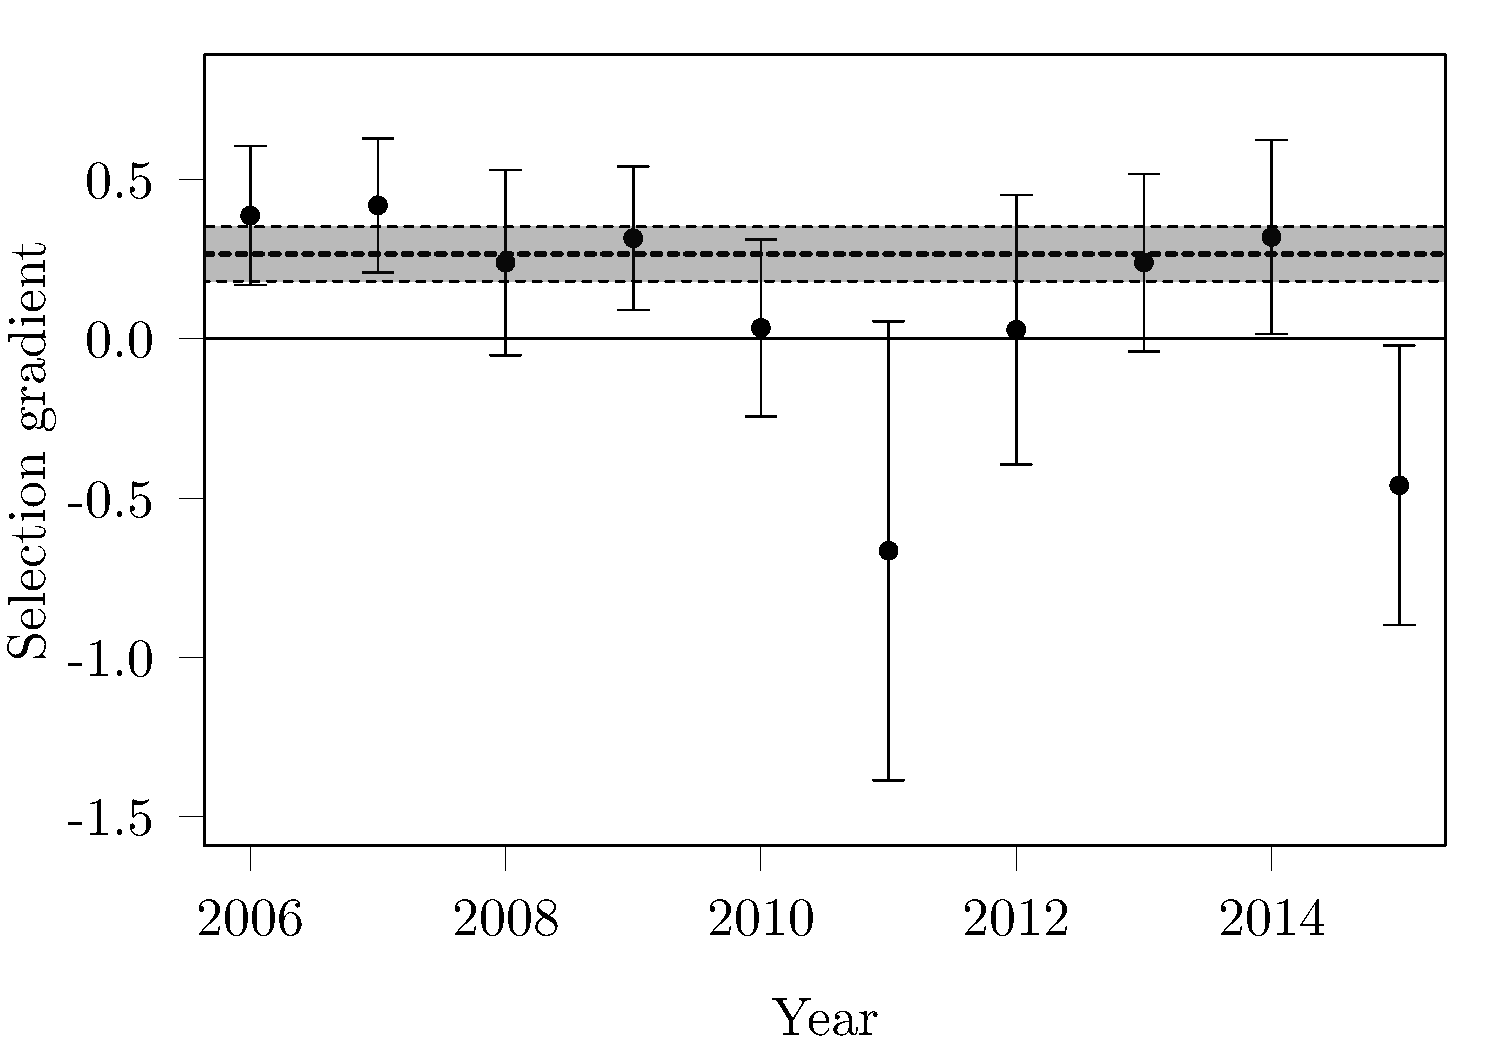
\includegraphics[width=\maxwidth]{figure/SelByYear-1} 
\begin{kframe}\begin{alltt}
\hlcom{#points(x=2006:2015,y=unlist(coefficients(mmRnoCorfitness)$Year["StMass"]), pch=17)}
\end{alltt}
\end{kframe}
\end{knitrout}

\begin{knitrout}
\definecolor{shadecolor}{rgb}{0.969, 0.969, 0.969}\color{fgcolor}\begin{kframe}
\begin{alltt}
\hlkwd{setPar}\hlstd{()}
\hlkwd{plot}\hlstd{(SelAByYearRho,} \hlkwc{x}\hlstd{=}\hlnum{2006}\hlopt{:}\hlnum{2015}\hlstd{,} \hlkwc{ylim}\hlstd{=}\hlkwd{c}\hlstd{(}\hlkwd{min}\hlstd{( CISelAByYearRho),} \hlkwd{max}\hlstd{( CISelAByYearRho)),} \hlkwc{xlab}\hlstd{=}\hlstr{"Year"}\hlstd{,} \hlkwc{ylab} \hlstd{=} \hlstr{"Selection gradient on $\textbackslash{}\textbackslash{}rho$"}\hlstd{,} \hlkwc{main} \hlstd{=} \hlstr{"\textbackslash{}\textbackslash{}textbf\{(B)\} Fertility selection"}\hlstd{)}
\hlkwd{abline}\hlstd{(}\hlkwc{h}\hlstd{=}\hlnum{0}\hlstd{)}
\hlkwd{arrows}\hlstd{(}\hlkwc{x0} \hlstd{=} \hlnum{2006}\hlopt{:}\hlnum{2015}\hlstd{,}\hlkwc{x1} \hlstd{=} \hlnum{2006}\hlopt{:}\hlnum{2015}\hlstd{,}\hlkwc{code} \hlstd{=} \hlnum{3}\hlstd{,} \hlkwc{y0} \hlstd{= CISelAByYearRho[}\hlnum{1}\hlstd{,],}
       \hlkwc{y1} \hlstd{= CISelAByYearRho[}\hlnum{2}\hlstd{,],} \hlkwc{angle} \hlstd{=} \hlnum{90}\hlstd{,}\hlkwc{length} \hlstd{=} \hlnum{0.1}\hlstd{)}
\hlkwd{abline}\hlstd{(}\hlkwc{h}\hlstd{=}\hlkwd{coefficients}\hlstd{(m0allRho)[}\hlnum{2}\hlstd{],} \hlkwc{lty}\hlstd{=}\hlnum{2}\hlstd{,} \hlkwc{lwd}\hlstd{=}\hlnum{5}\hlstd{)}
\hlstd{sm0allRho} \hlkwb{<-} \hlkwd{summary}\hlstd{(m0allRho)}
\hlstd{lowm0allRho} \hlkwb{<-} \hlkwd{coefficients}\hlstd{(m0allRho)[}\hlnum{2}\hlstd{]}\hlopt{+}\hlnum{1.96}\hlopt{*}\hlstd{sm0allRho}\hlopt{$}\hlstd{coefficients[}\hlnum{2}\hlstd{,}\hlnum{2}\hlstd{]}
\hlstd{highm0allRho} \hlkwb{<-} \hlkwd{coefficients}\hlstd{(m0allRho)[}\hlnum{2}\hlstd{]}\hlopt{-}\hlnum{1.96}\hlopt{*}\hlstd{sm0allRho}\hlopt{$}\hlstd{coefficients[}\hlnum{2}\hlstd{,}\hlnum{2}\hlstd{]}
\hlkwd{polygon}\hlstd{(}\hlkwc{x}\hlstd{=}\hlkwd{c}\hlstd{(}\hlnum{2005}\hlstd{,}\hlnum{2016}\hlstd{,}\hlnum{2016}\hlstd{,}\hlnum{2005}\hlstd{),}\hlkwc{y}\hlstd{=}\hlkwd{c}\hlstd{(lowm0allRho,lowm0allRho, highm0allRho, highm0allRho),}
        \hlkwc{fillOddEven} \hlstd{=} \hlnum{TRUE}\hlstd{,} \hlkwc{col}\hlstd{=}\hlkwd{rgb}\hlstd{(}\hlnum{0.1}\hlstd{,}\hlnum{0.1}\hlstd{,}\hlnum{0.1}\hlstd{,}\hlnum{0.5}\hlstd{),} \hlkwc{lty}\hlstd{=}\hlnum{2}\hlstd{)}
\end{alltt}
\end{kframe}
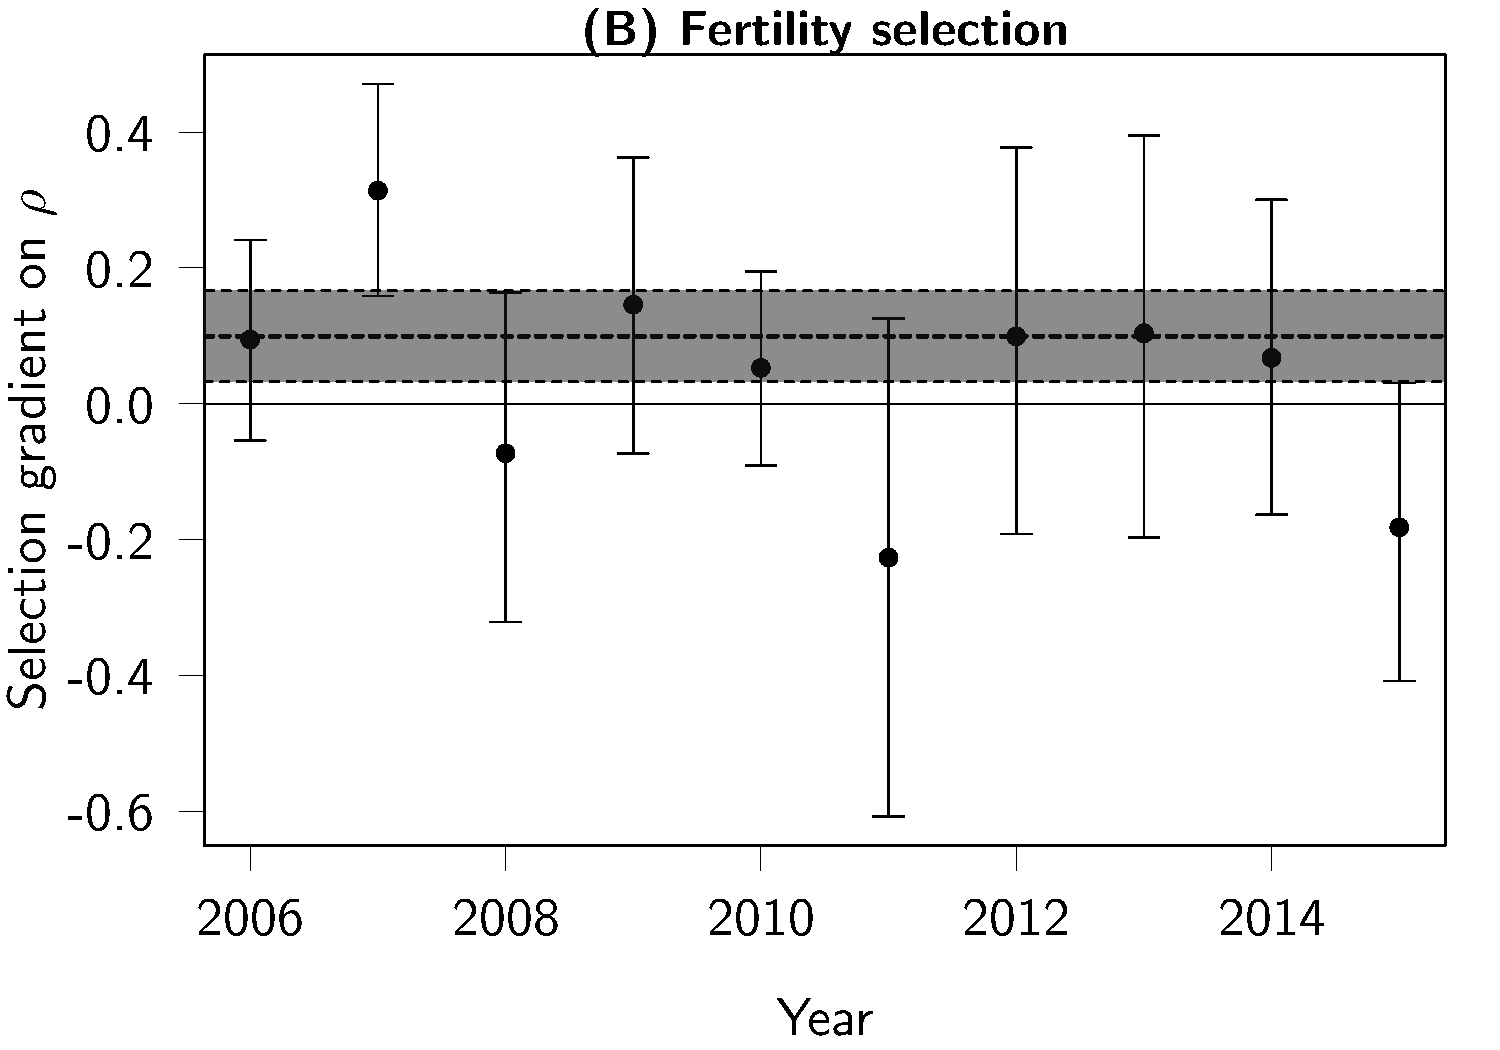
\includegraphics[width=\maxwidth]{figure/SelByYearRho-1} 

\end{knitrout}


\begin{knitrout}
\definecolor{shadecolor}{rgb}{0.969, 0.969, 0.969}\color{fgcolor}\begin{kframe}
\begin{alltt}
\hlkwd{setPar}\hlstd{()}
\hlkwd{plot}\hlstd{(SelAByYearPhi,} \hlkwc{x}\hlstd{=}\hlnum{2006}\hlopt{:}\hlnum{2015}\hlstd{,} \hlkwc{ylim}\hlstd{=}\hlkwd{c}\hlstd{(}\hlkwd{min}\hlstd{( CISelAByYearPhi,} \hlkwc{na.rm}\hlstd{=}\hlnum{TRUE}\hlstd{),} \hlkwd{max}\hlstd{( CISelAByYearPhi,} \hlkwc{na.rm}\hlstd{=}\hlnum{TRUE}\hlstd{)),} \hlkwc{xlab}\hlstd{=}\hlstr{"Year"}\hlstd{,} \hlkwc{ylab} \hlstd{=} \hlstr{"Selection gradient on $\textbackslash{}\textbackslash{}phi$"}\hlstd{,} \hlkwc{main} \hlstd{=} \hlstr{"\textbackslash{}\textbackslash{}textbf\{(C)\} Viability selection"}\hlstd{)}
\hlkwd{abline}\hlstd{(}\hlkwc{h}\hlstd{=}\hlnum{0}\hlstd{)}
\hlkwd{arrows}\hlstd{(}\hlkwc{x0} \hlstd{=} \hlnum{2006}\hlopt{:}\hlnum{2015}\hlstd{,}\hlkwc{x1} \hlstd{=} \hlnum{2006}\hlopt{:}\hlnum{2015}\hlstd{,}\hlkwc{code} \hlstd{=} \hlnum{3}\hlstd{,} \hlkwc{y0} \hlstd{= CISelAByYearPhi[}\hlnum{1}\hlstd{,],}
       \hlkwc{y1} \hlstd{= CISelAByYearPhi[}\hlnum{2}\hlstd{,],} \hlkwc{angle} \hlstd{=} \hlnum{90}\hlstd{,}\hlkwc{length} \hlstd{=} \hlnum{0.1}\hlstd{)}
\hlkwd{abline}\hlstd{(}\hlkwc{h}\hlstd{=}\hlkwd{coefficients}\hlstd{(m0allphi)[}\hlnum{2}\hlstd{],} \hlkwc{lty}\hlstd{=}\hlnum{2}\hlstd{,} \hlkwc{lwd}\hlstd{=}\hlnum{5}\hlstd{)}
\hlstd{lowm0allphi} \hlkwb{<-} \hlkwd{coefficients}\hlstd{(m0allphi)[}\hlnum{2}\hlstd{]}\hlopt{+}\hlnum{1.96}\hlopt{*}\hlstd{sm0allphi}\hlopt{$}\hlstd{coefficients[}\hlnum{2}\hlstd{,}\hlnum{2}\hlstd{]}
\hlstd{highm0allphi} \hlkwb{<-} \hlkwd{coefficients}\hlstd{(m0allphi)[}\hlnum{2}\hlstd{]}\hlopt{-}\hlnum{1.96}\hlopt{*}\hlstd{sm0allphi}\hlopt{$}\hlstd{coefficients[}\hlnum{2}\hlstd{,}\hlnum{2}\hlstd{]}
\hlkwd{polygon}\hlstd{(}\hlkwc{x}\hlstd{=}\hlkwd{c}\hlstd{(}\hlnum{2005}\hlstd{,}\hlnum{2016}\hlstd{,}\hlnum{2016}\hlstd{,}\hlnum{2005}\hlstd{),}\hlkwc{y}\hlstd{=}\hlkwd{c}\hlstd{(lowm0allphi,lowm0allphi, highm0allphi, highm0allphi),}
        \hlkwc{fillOddEven} \hlstd{=} \hlnum{TRUE}\hlstd{,} \hlkwc{col}\hlstd{=}\hlkwd{rgb}\hlstd{(}\hlnum{0.1}\hlstd{,}\hlnum{0.1}\hlstd{,}\hlnum{0.1}\hlstd{,}\hlnum{0.5}\hlstd{),} \hlkwc{lty}\hlstd{=}\hlnum{2} \hlstd{)}
\end{alltt}
\end{kframe}
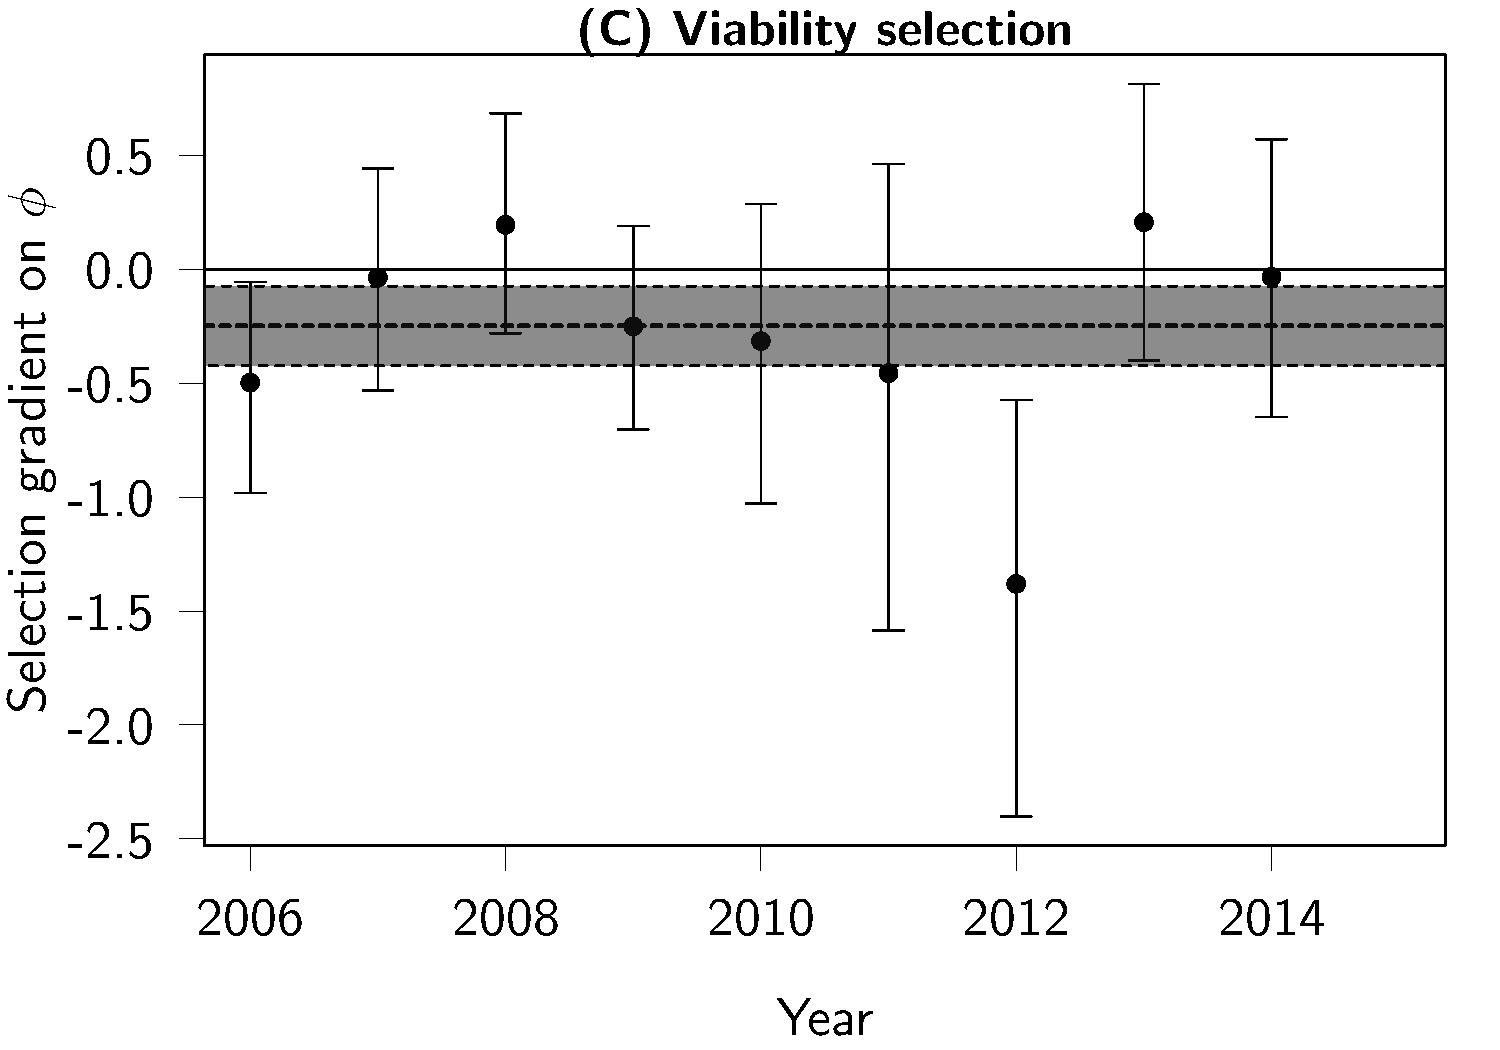
\includegraphics[width=\maxwidth]{figure/SelByYearPhi-1} 

\end{knitrout}
Correlation fertility viability
\begin{knitrout}
\definecolor{shadecolor}{rgb}{0.969, 0.969, 0.969}\color{fgcolor}\begin{kframe}
\begin{alltt}
\hlkwd{cor.test}\hlstd{(YearPheno}\hlopt{$}\hlstd{Phi,YearPheno}\hlopt{$}\hlstd{Rho)}
\end{alltt}
\begin{verbatim}
## 
## 	Pearson's product-moment correlation
## 
## data:  YearPheno$Phi and YearPheno$Rho
## t = -1.9473, df = 1292, p-value = 0.05171
## alternative hypothesis: true correlation is not equal to 0
## 95 percent confidence interval:
##  -0.1082724891  0.0003989614
## sample estimates:
##         cor 
## -0.05409695
\end{verbatim}
\end{kframe}
\end{knitrout}

\begin{knitrout}
\definecolor{shadecolor}{rgb}{0.969, 0.969, 0.969}\color{fgcolor}\begin{kframe}
\begin{alltt}
\hlstd{rounding} \hlkwb{<-} \hlnum{3}

\hlstd{BetaGlm}\hlkwb{<-} \hlkwd{c}\hlstd{(}\hlkwd{paste}\hlstd{(}\hlkwd{round}\hlstd{(sm0all}\hlopt{$}\hlstd{coefficients[}\hlnum{2}\hlstd{,}\hlnum{1}\hlstd{],rounding),}\hlstr{" ("}\hlstd{,}\hlkwd{round}\hlstd{(sm0all}\hlopt{$}\hlstd{coefficients[}\hlnum{2}\hlstd{,}\hlnum{2}\hlstd{],rounding ),}\hlstr{")"}\hlstd{,}\hlkwc{sep}\hlstd{=}\hlstr{""}\hlstd{),}
            \hlkwd{paste}\hlstd{(}\hlkwd{round}\hlstd{(sm0allRho}\hlopt{$}\hlstd{coefficients[}\hlnum{2}\hlstd{,}\hlnum{1}\hlstd{],rounding),}\hlstr{" ("}\hlstd{,}\hlkwd{round}\hlstd{(sm0allRho}\hlopt{$}\hlstd{coefficients[}\hlnum{2}\hlstd{,}\hlnum{2}\hlstd{],rounding ),}\hlstr{")"}\hlstd{,}\hlkwc{sep}\hlstd{=}\hlstr{""}\hlstd{),}
            \hlkwd{paste}\hlstd{(}\hlkwd{round}\hlstd{(sm0allphi}\hlopt{$}\hlstd{coefficients[}\hlnum{2}\hlstd{,}\hlnum{1}\hlstd{],rounding),}\hlstr{" ("}\hlstd{,}\hlkwd{round}\hlstd{(sm0allphi}\hlopt{$}\hlstd{coefficients[}\hlnum{2}\hlstd{,}\hlnum{2}\hlstd{],rounding ),}\hlstr{")"}\hlstd{,}\hlkwc{sep}\hlstd{=}\hlstr{""}\hlstd{))}

\hlstd{SDyears} \hlkwb{<-} \hlkwd{c}\hlstd{(}\hlkwd{sd}\hlstd{(SelAByYear),}\hlkwd{sd}\hlstd{(SelAByYearRho),}\hlkwd{sd}\hlstd{(SelAByYearPhi,} \hlkwc{na.rm}\hlstd{=}\hlnum{TRUE}\hlstd{))}
\hlstd{SEyears} \hlkwb{<-} \hlkwd{c}\hlstd{(}\hlkwd{mean}\hlstd{(SeSelAByYear),} \hlkwd{mean}\hlstd{(SeSelAByYearRho),}\hlkwd{mean}\hlstd{(SeSelAByYearPhi,}\hlkwc{na.rm}\hlstd{=T))}
\hlstd{BetaGLMM} \hlkwb{<-} \hlkwd{c}\hlstd{(}\hlkwd{paste}\hlstd{(}\hlkwd{round}\hlstd{(smmARnoCorfitness}\hlopt{$}\hlstd{coefficients[}\hlnum{2}\hlstd{,}\hlnum{1}\hlstd{],rounding),}\hlstr{" ("}\hlstd{,}\hlkwd{round}\hlstd{(smmARnoCorfitness}\hlopt{$}\hlstd{coefficients[}\hlnum{2}\hlstd{,}\hlnum{2}\hlstd{],rounding ),}\hlstr{")"}\hlstd{,}\hlkwc{sep}\hlstd{=}\hlstr{""}\hlstd{),}
            \hlkwd{paste}\hlstd{(}\hlkwd{round}\hlstd{(smmRnoCorrho}\hlopt{$}\hlstd{coefficients[}\hlnum{2}\hlstd{,}\hlnum{1}\hlstd{],rounding),}\hlstr{" ("}\hlstd{,}\hlkwd{round}\hlstd{(smmRnoCorrho}\hlopt{$}\hlstd{coefficients[}\hlnum{2}\hlstd{,}\hlnum{2}\hlstd{],rounding ),}\hlstr{")"}\hlstd{,}\hlkwc{sep}\hlstd{=}\hlstr{""}\hlstd{),}
            \hlkwd{paste}\hlstd{(}\hlkwd{round}\hlstd{(smmRnoCorphi}\hlopt{$}\hlstd{coefficients[}\hlnum{2}\hlstd{,}\hlnum{1}\hlstd{],rounding),}\hlstr{" ("}\hlstd{,}\hlkwd{round}\hlstd{(smmRnoCorphi}\hlopt{$}\hlstd{coefficients[}\hlnum{2}\hlstd{,}\hlnum{2}\hlstd{],rounding ),}\hlstr{")"}\hlstd{,}\hlkwc{sep}\hlstd{=}\hlstr{""}\hlstd{))}
\hlstd{SigmaA} \hlkwb{<-} \hlkwd{c}\hlstd{(}\hlkwd{sqrt}\hlstd{(}\hlkwd{as.numeric}\hlstd{(smmARnoCorfitness}\hlopt{$}\hlstd{varcor}\hlopt{$}\hlstd{Year.1)),}
            \hlkwd{sqrt}\hlstd{(}\hlkwd{as.numeric}\hlstd{(smmRnoCorrho}\hlopt{$}\hlstd{varcor}\hlopt{$}\hlstd{Year.1)),}
\hlkwd{sqrt}\hlstd{(}\hlkwd{as.numeric}\hlstd{(smmRnoCorphi}\hlopt{$}\hlstd{varcor}\hlopt{$}\hlstd{Year.1)))}
\hlstd{SigRat} \hlkwb{<-} \hlkwd{c}\hlstd{(}\hlkwd{sqrt}\hlstd{(}\hlkwd{as.numeric}\hlstd{(smmARnoCorfitness}\hlopt{$}\hlstd{varcor}\hlopt{$}\hlstd{Year.1))}\hlopt{/}\hlstd{smmARnoCorfitness}\hlopt{$}\hlstd{coefficients[}\hlnum{2}\hlstd{,}\hlnum{1}\hlstd{],}
            \hlkwd{sqrt}\hlstd{(}\hlkwd{as.numeric}\hlstd{(smmRnoCorrho}\hlopt{$}\hlstd{varcor}\hlopt{$}\hlstd{Year.1))}\hlopt{/}\hlstd{smmRnoCorrho}\hlopt{$}\hlstd{coefficients[}\hlnum{2}\hlstd{,}\hlnum{1}\hlstd{],}
\hlkwd{sqrt}\hlstd{(}\hlkwd{as.numeric}\hlstd{(smmRnoCorphi}\hlopt{$}\hlstd{varcor}\hlopt{$}\hlstd{Year.1))}\hlopt{/}\hlstd{smmRnoCorphi}\hlopt{$}\hlstd{coefficients[}\hlnum{2}\hlstd{,}\hlnum{1}\hlstd{])}

\hlstd{psigmaA} \hlkwb{<-} \hlkwd{c}\hlstd{(fitnessAanova}\hlopt{$}\hlstd{`Pr(>Chisq)`[}\hlnum{2}\hlstd{]}\hlopt{/}\hlnum{2}\hlstd{, RhoAanova}\hlopt{$}\hlstd{`Pr(>Chisq)`[}\hlnum{2}\hlstd{]}\hlopt{/}\hlnum{2}\hlstd{, PhiAanova}\hlopt{$}\hlstd{`Pr(>Chisq)`[}\hlnum{2}\hlstd{]}\hlopt{/}\hlnum{2}\hlstd{)}
\hlstd{confsigma} \hlkwb{<-} \hlkwd{c}\hlstd{(}\hlkwd{paste}\hlstd{(}\hlstr{"["}\hlstd{,}\hlkwd{round}\hlstd{(CImmARnoCorfitness[}\hlnum{2}\hlstd{,}\hlnum{1}\hlstd{],rounding),}\hlstr{";"}\hlstd{,}\hlkwd{round}\hlstd{(CImmARnoCorfitness[}\hlnum{2}\hlstd{,}\hlnum{2}\hlstd{],rounding),}\hlstr{"]"}\hlstd{,}\hlkwc{sep}\hlstd{=}\hlstr{""}\hlstd{),}
               \hlkwd{paste}\hlstd{(}\hlstr{"["}\hlstd{,}\hlkwd{round}\hlstd{(CImmRnoCorrho[}\hlnum{2}\hlstd{,}\hlnum{1}\hlstd{],rounding),}\hlstr{";"}\hlstd{,}\hlkwd{round}\hlstd{(CImmRnoCorrho[}\hlnum{2}\hlstd{,}\hlnum{2}\hlstd{],rounding),}\hlstr{"]"}\hlstd{,}\hlkwc{sep}\hlstd{=}\hlstr{""}\hlstd{),}
               \hlkwd{paste}\hlstd{(}\hlstr{"["}\hlstd{,}\hlkwd{round}\hlstd{(CImmRnoCorphi[}\hlnum{2}\hlstd{,}\hlnum{1}\hlstd{],rounding),}\hlstr{";"}\hlstd{,}\hlkwd{round}\hlstd{(CImmRnoCorphi[}\hlnum{2}\hlstd{,}\hlnum{2}\hlstd{],rounding),}\hlstr{"]"}\hlstd{,}\hlkwc{sep}\hlstd{=}\hlstr{""}\hlstd{))}

\hlstd{TabSel} \hlkwb{<-} \hlkwd{data.frame}\hlstd{(}\hlkwc{BetaGlm} \hlstd{= BetaGlm,} \hlkwc{B}\hlstd{=SDyears,} \hlkwc{C}\hlstd{=SEyears ,} \hlkwc{D}\hlstd{=BetaGLMM ,} \hlkwc{E}\hlstd{=SigmaA,} \hlkwc{DD} \hlstd{=confsigma,} \hlkwc{EE} \hlstd{=psigmaA,} \hlkwc{FF}\hlstd{=SigRat)}
\end{alltt}
\end{kframe}
\end{knitrout}

% latex table generated in R 3.2.4 by xtable 1.8-2 package
% Fri May 13 17:33:12 2016
\begin{table}[ht]
\centering
\caption{} 
\label{Test_table}
\begingroup\footnotesize
\begin{tabular}{lrrlrlrr}
  0.082 (0.028) & 0.167 & 0.097 & 0.036 (0.044) & 0.117 & [0.063;0.218] & 8.1E-06 & 3.241 \\ 
  0.1 (0.034) & 0.160 & 0.117 & 0.052 (0.044) & 0.111 & [0.053;0.212] & 2.5E-04 & 2.145 \\ 
  -0.248 (0.089) & 0.484 & 0.319 & -0.217 (0.098) & 0.109 & [0;0.425] & 3.6E-01 & -0.501 \\ 
  \end{tabular}
\endgroup
\end{table}


%' 
%' <<EvolSmooth,dev="tikz",fig.height=7,fig.width=10>>=
%' setPar()
%' plot(x=0,xlim=c(2006,2015),ylim=c(-1,1),type="n", xlab="Year",ylab="Breeding values for mass (g)")
%' trashidontwantyou<-lapply(bvplotlist, function(x){lines(x[,1],x[,2], col=rgb(0.1,0.1,0.1,alpha = 0.1))})
%' @
%' 
 
\begin{knitrout}
\definecolor{shadecolor}{rgb}{0.969, 0.969, 0.969}\color{fgcolor}\begin{kframe}
\begin{alltt}
\hlstd{szgr} \hlkwb{<-} \hlnum{2}
\hlstd{szax} \hlkwb{<-} \hlnum{1.3}
\hlstd{marr} \hlkwb{<-} \hlkwd{c}\hlstd{(}\hlnum{4}\hlstd{,} \hlnum{4}\hlstd{,} \hlnum{1}\hlstd{,} \hlnum{1}\hlstd{)} \hlopt{+} \hlnum{0.1}
\hlkwd{par}\hlstd{(}\hlkwc{las}\hlstd{=}\hlnum{1}\hlstd{,}\hlkwc{mar}\hlstd{=marr,} \hlkwc{cex}\hlstd{=szgr,} \hlkwc{cex.lab}\hlstd{=szax ,} \hlkwc{cex.axis}\hlstd{=szax,} \hlkwc{lwd}\hlstd{=}\hlnum{2} \hlstd{,} \hlkwc{las}\hlstd{=}\hlnum{1}\hlstd{)}

\hlstd{bbv} \hlkwb{<-} \hlkwd{boxplot}\hlstd{(bvpairwise,}\hlkwc{ylab}\hlstd{=}\hlstr{"Change in breeding values (g)"}\hlstd{,} \hlkwc{xlab}\hlstd{=}\hlstr{"Year"}\hlstd{,} \hlkwc{range} \hlstd{=} \hlnum{1}\hlstd{,}\hlkwc{cex}\hlstd{=}\hlnum{1}\hlstd{)}
\hlstd{bbv}\hlopt{$}\hlstd{stats}
\end{alltt}
\begin{verbatim}
##              [,1]         [,2]         [,3]         [,4]         [,5]
## [1,] -0.280501568 -0.257383635 -0.347173588 -0.267832000 -0.357132486
## [2,] -0.143366410 -0.087176846 -0.178386364 -0.095028840 -0.114692786
## [3,] -0.067520536 -0.003132208 -0.094707610  0.002214962  0.005447066
## [4,] -0.003739138  0.086721131 -0.008337006  0.082918931  0.130138872
## [5,]  0.134012211  0.260359089  0.161244353  0.260692898  0.371425991
##            [,6]        [,7]         [,8]        [,9]
## [1,] -0.8321504 -0.17794910 -0.382623528 -0.29096950
## [2,] -0.4928537  0.06339068 -0.130565493 -0.07342106
## [3,] -0.3192183  0.19033674 -0.004056911  0.03549705
## [4,] -0.1519085  0.31816724  0.122591670  0.14822783
## [5,]  0.1872504  0.57031481  0.374995899  0.36644027
\end{verbatim}
\begin{alltt}
\hlstd{bbv}\hlopt{$}\hlstd{group}
\end{alltt}
\begin{verbatim}
##   [1] 1 1 1 1 1 1 1 1 1 1 1 1 1 1 1 1 1 1 1 1 1 1 1 1 1 1 1 1 1 1 1 1 1 1 1
##  [36] 1 1 1 1 1 1 1 1 1 2 2 2 2 2 2 2 2 2 2 2 2 2 2 2 2 2 2 2 2 2 2 2 2 2 2
##  [71] 2 2 2 2 2 2 2 2 2 2 2 3 3 3 3 3 3 3 3 3 3 3 3 3 3 3 3 3 3 3 3 3 3 3 3
## [106] 3 3 3 3 3 3 3 3 3 3 4 4 4 4 4 4 4 4 4 4 4 4 4 4 4 4 4 4 4 4 4 4 4 4 4
## [141] 4 4 4 4 4 4 4 4 4 4 4 4 4 4 4 5 5 5 5 5 5 5 5 5 5 5 5 5 5 5 5 5 5 5 5
## [176] 5 5 5 5 5 5 5 5 5 5 5 5 5 5 5 5 5 6 6 6 6 6 6 6 6 6 6 6 6 6 6 6 6 6 6
## [211] 6 6 6 6 6 6 6 6 6 6 6 6 6 6 6 6 6 6 6 6 6 6 6 6 6 6 7 7 7 7 7 7 7 7 7
## [246] 7 7 7 7 7 7 7 7 7 7 7 7 7 7 7 7 7 7 7 7 7 7 7 7 7 7 7 7 7 7 7 8 8 8 8
## [281] 8 8 8 8 8 8 8 8 8 8 8 8 8 8 8 8 8 8 8 8 8 8 8 8 8 8 8 8 9 9 9 9 9 9 9
## [316] 9 9 9 9 9 9 9 9 9 9 9 9 9 9 9 9 9 9 9 9 9 9 9 9 9 9 9 9 9 9 9 9 9 9 9
## [351] 9
\end{verbatim}
\begin{alltt}
\hlkwd{abline}\hlstd{(}\hlkwc{h}\hlstd{=}\hlnum{0}\hlstd{)}
\end{alltt}
\end{kframe}
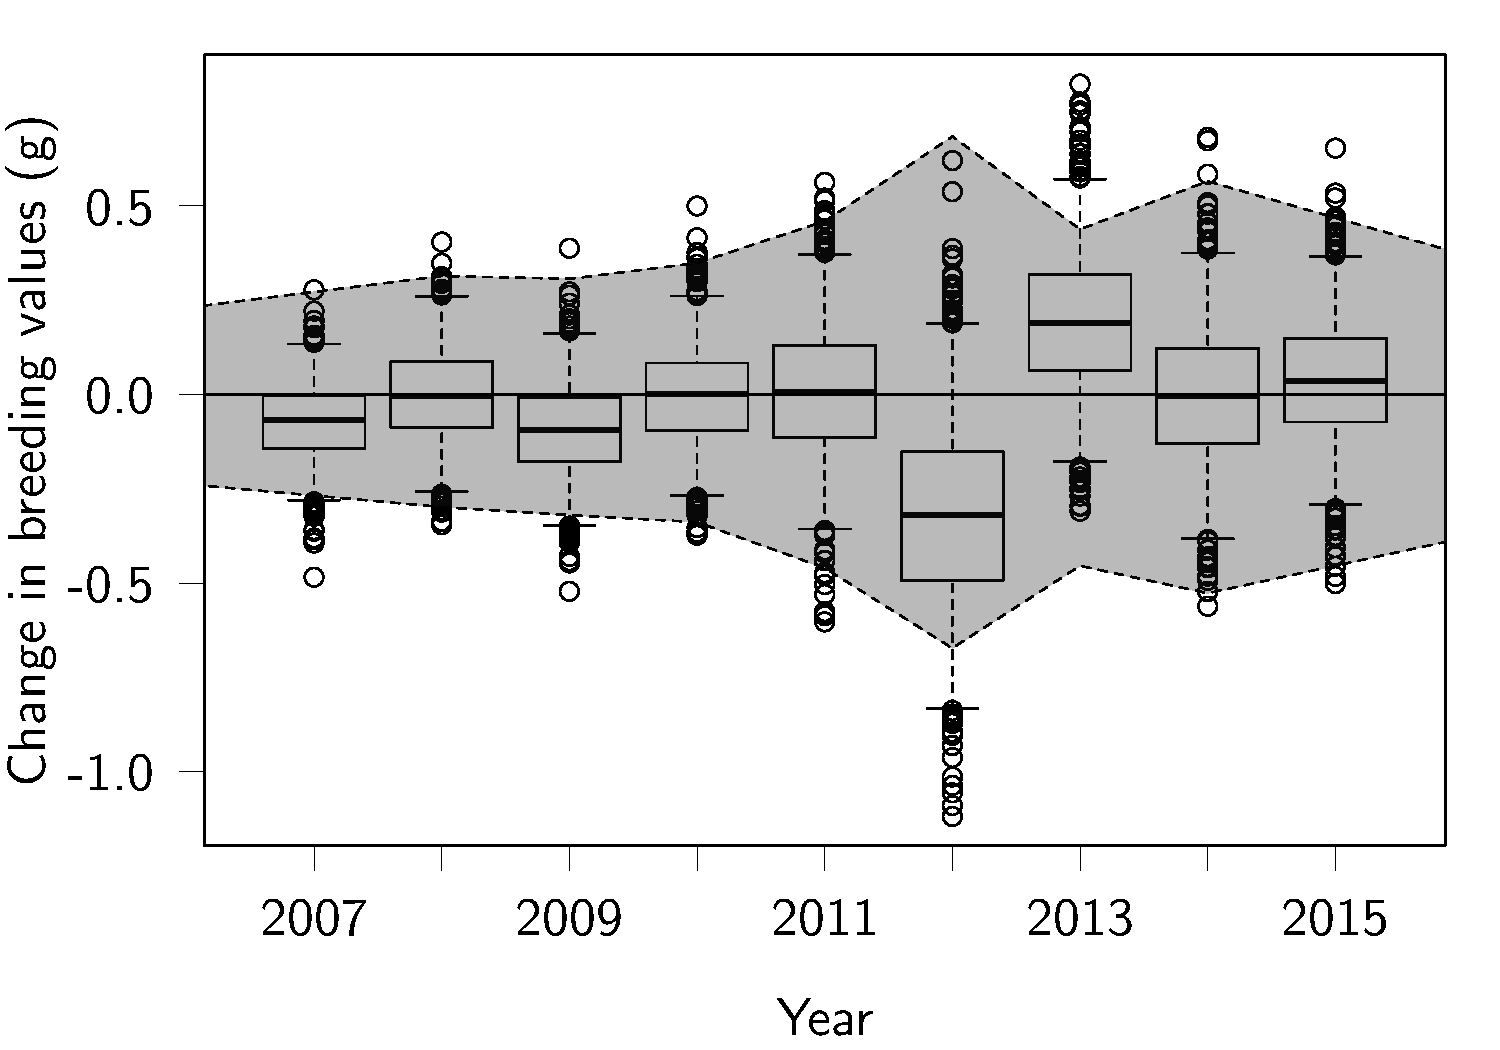
\includegraphics[width=\maxwidth]{figure/EvolDiff-1} 
\begin{kframe}\begin{alltt}
\hlkwd{density}\hlstd{(bvpairwise[,}\hlnum{1}\hlstd{])}
\end{alltt}
\begin{verbatim}
## 
## Call:
## 	density.default(x = bvpairwise[, 1])
## 
## Data: bvpairwise[, 1] (1000 obs.);	Bandwidth 'bw' = 0.02343
## 
##        x                 y           
##  Min.   :-0.5547   Min.   :0.000192  
##  1st Qu.:-0.3292   1st Qu.:0.018199  
##  Median :-0.1036   Median :0.424183  
##  Mean   :-0.1036   Mean   :1.107278  
##  3rd Qu.: 0.1219   3rd Qu.:2.109751  
##  Max.   : 0.3475   Max.   :3.900320
\end{verbatim}
\end{kframe}
\end{knitrout}

\begin{knitrout}
\definecolor{shadecolor}{rgb}{0.969, 0.969, 0.969}\color{fgcolor}\begin{kframe}
\begin{alltt}
\hlkwd{setPar}\hlstd{()}
\hlkwd{par}\hlstd{(}\hlkwc{mar}\hlstd{=}\hlkwd{c}\hlstd{(}\hlnum{4}\hlstd{,} \hlnum{6}\hlstd{,} \hlnum{1}\hlstd{,} \hlnum{1}\hlstd{)} \hlopt{+} \hlnum{0.1}\hlstd{)}
\hlstd{Betas} \hlkwb{<-} \hlkwd{matrix}\hlstd{(}\hlkwd{sapply}\hlstd{(}\hlkwc{X} \hlstd{=} \hlkwd{list}\hlstd{(BetaP1, BetaE1, BetaG1, BetaP2, BetaE2, BetaG2), posterior.mode),}\hlkwc{nrow} \hlstd{=}\hlnum{3}\hlstd{,} \hlkwc{byrow}\hlstd{=}\hlnum{FALSE}\hlstd{)}
\hlstd{BetasCI} \hlkwb{<-} \hlkwd{sapply}\hlstd{(}\hlkwc{X} \hlstd{=} \hlkwd{list}\hlstd{(BetaP1, BetaE1, BetaG1, BetaP2, BetaE2, BetaG2), HPDinterval)}

\hlstd{x} \hlkwb{<-} \hlkwd{barplot}\hlstd{(Betas,} \hlkwc{beside}\hlstd{=}\hlnum{TRUE}\hlstd{,} \hlkwc{ylim}\hlstd{=}\hlkwd{c}\hlstd{(}\hlkwd{min}\hlstd{(BetasCI),}\hlkwd{max}\hlstd{(BetasCI)),}\hlkwc{names.arg} \hlstd{=} \hlkwd{c}\hlstd{(}\hlstr{"Postive selection years"}\hlstd{,}\hlstr{"Negative selection years"}\hlstd{),} \hlkwc{legend.text} \hlstd{=} \hlkwd{c}\hlstd{(}\hlstr{"Phenotypic"}\hlstd{,}\hlstr{"Environmental"}\hlstd{,}\hlstr{"Genetic"}\hlstd{))}
\hlkwd{abline}\hlstd{(}\hlkwc{h}\hlstd{=}\hlnum{0}\hlstd{)}
\hlkwd{arrows}\hlstd{(}\hlkwc{x0} \hlstd{= x,} \hlkwc{y0}\hlstd{=BetasCI[}\hlnum{1}\hlstd{,],}\hlkwc{y1}\hlstd{=BetasCI[}\hlnum{2}\hlstd{,],}\hlkwc{angle} \hlstd{=} \hlnum{90}\hlstd{,}\hlkwc{code} \hlstd{=} \hlnum{3}\hlstd{)}
\hlkwd{mtext}\hlstd{(}\hlkwc{side}\hlstd{=}\hlnum{2}\hlstd{,} \hlstr{"Selection gradients"}\hlstd{,} \hlkwc{line}\hlstd{=}\hlnum{4}\hlstd{,} \hlkwc{las}\hlstd{=}\hlnum{0}\hlstd{,} \hlkwc{cex}\hlstd{=szax}\hlopt{*}\hlstd{szgr)}
\end{alltt}
\end{kframe}
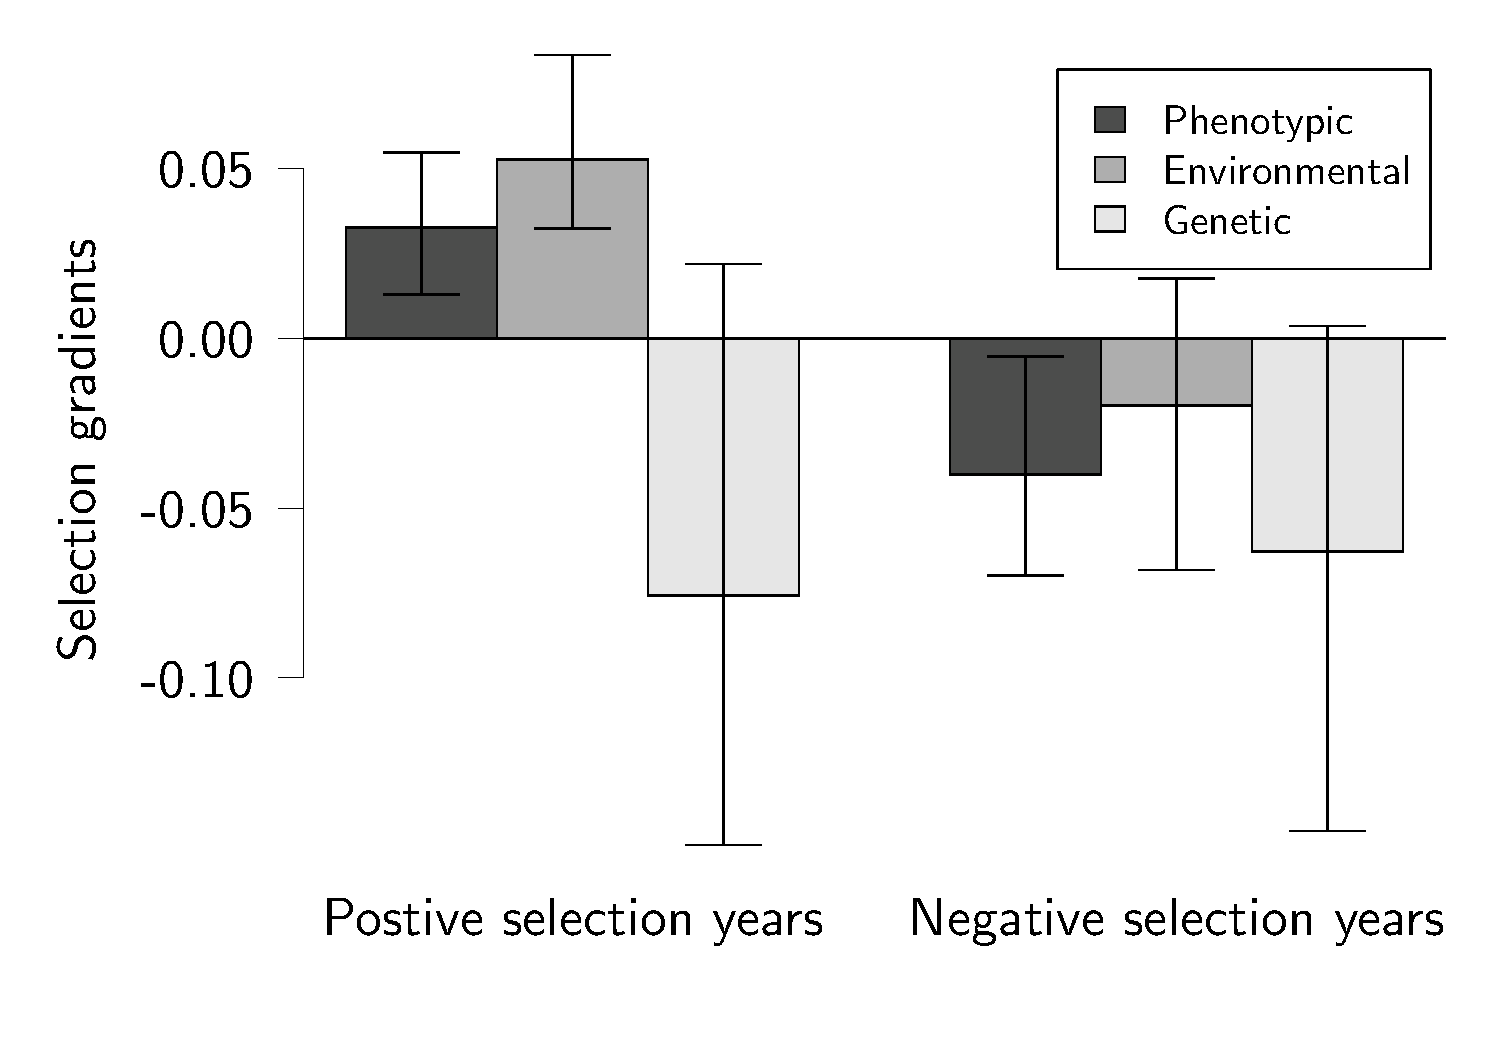
\includegraphics[width=\maxwidth]{figure/Betas-1} 

\end{knitrout}

\begin{knitrout}
\definecolor{shadecolor}{rgb}{0.969, 0.969, 0.969}\color{fgcolor}\begin{kframe}
\begin{alltt}
\hlkwd{posterior.mode}\hlstd{(BetaG1} \hlopt{-} \hlstd{BetaE1)}
\end{alltt}
\begin{verbatim}
##       var1 
## -0.1234186
\end{verbatim}
\begin{alltt}
\hlkwd{HPDinterval}\hlstd{(BetaG1} \hlopt{-} \hlstd{BetaE1)}
\end{alltt}
\begin{verbatim}
##           lower       upper
## var1 -0.2180723 -0.02770633
## attr(,"Probability")
## [1] 0.95
\end{verbatim}
\begin{alltt}
\hlkwd{mean}\hlstd{((BetaG1} \hlopt{-} \hlstd{BetaE1)}\hlopt{>}\hlnum{0}\hlstd{)}\hlopt{*}\hlnum{2}
\end{alltt}
\begin{verbatim}
## [1] 0.006
\end{verbatim}
\begin{alltt}
\hlkwd{posterior.mode}\hlstd{(BetaG2} \hlopt{-} \hlstd{BetaE2)}
\end{alltt}
\begin{verbatim}
##         var1 
## -0.009610168
\end{verbatim}
\begin{alltt}
\hlkwd{HPDinterval}\hlstd{(BetaG2} \hlopt{-} \hlstd{BetaE2)}
\end{alltt}
\begin{verbatim}
##           lower      upper
## var1 -0.1379426 0.05755331
## attr(,"Probability")
## [1] 0.95
\end{verbatim}
\begin{alltt}
\hlkwd{mean}\hlstd{((BetaG2} \hlopt{-} \hlstd{BetaE2)}\hlopt{>}\hlnum{0}\hlstd{)}\hlopt{*}\hlnum{2}
\end{alltt}
\begin{verbatim}
## [1] 0.424
\end{verbatim}
\begin{alltt}
\hlkwd{posterior.mode}\hlstd{(BetaE1} \hlopt{-} \hlstd{BetaE2)}
\end{alltt}
\begin{verbatim}
##       var1 
## 0.07575993
\end{verbatim}
\begin{alltt}
\hlkwd{HPDinterval}\hlstd{(BetaE1} \hlopt{-} \hlstd{BetaE2)}
\end{alltt}
\begin{verbatim}
##           lower     upper
## var1 0.03828845 0.1372658
## attr(,"Probability")
## [1] 0.95
\end{verbatim}
\begin{alltt}
\hlkwd{mean}\hlstd{((BetaE1} \hlopt{-} \hlstd{BetaE2)}\hlopt{<}\hlnum{0}\hlstd{)}\hlopt{*}\hlnum{2}
\end{alltt}
\begin{verbatim}
## [1] 0
\end{verbatim}
\begin{alltt}
\hlkwd{posterior.mode}\hlstd{(BetaG1} \hlopt{-} \hlstd{BetaG2)}
\end{alltt}
\begin{verbatim}
##         var1 
## -0.003689573
\end{verbatim}
\begin{alltt}
\hlkwd{HPDinterval}\hlstd{(BetaG1} \hlopt{-} \hlstd{BetaG2)}
\end{alltt}
\begin{verbatim}
##            lower      upper
## var1 -0.08005378 0.07575714
## attr(,"Probability")
## [1] 0.95
\end{verbatim}
\begin{alltt}
\hlkwd{mean}\hlstd{((BetaG1} \hlopt{-} \hlstd{BetaG2)}\hlopt{>}\hlnum{0}\hlstd{)}\hlopt{*}\hlnum{2}
\end{alltt}
\begin{verbatim}
## [1] 0.908
\end{verbatim}
\end{kframe}
\end{knitrout}

\end{document}
